% uid: ""
% school: "college"
% level: "7eme"
% chapter: "التناظر المحوري"
% chapter_slug: "symetrie-axiale"
% title: "مناظرة دائرة ومستقيم"
% difficulty: "Facile"
% tags: ["symetrie-axiale", "cercle", "droite-perpendiculaire"]
% provenance: "own"
% batch: "2026-11-27-symetrie-axiale-7eme"
% Exercice 8/10 de la série 7ème « التناظر المحوري » (statement + \axsol + solution). Compiler avec XeLaTeX + axiomath.sty (+ axiomaths-logo.png).
\documentclass[12pt,a4paper]{article}
\usepackage[level=7b,color=0F766E]{axiomath}
\newcommand{\cm}{\,\mathrm{cm}}
\axsetup{title={التناظر المحوري}, corrige}

\begin{document}

\begin{corr}[title={مناظرة دائرة ومستقيم}, stars=2, source={Axiomaths}]
$\Delta$ مستقيم و $O$ نقطة تبعد $3\cm$ عن $\Delta$. $\mathcal{C}$ الدائرة التي مركزها $O$ وشعاعها $2\cm$.
\begin{enumerate}
  \item ابنِ $O'$ مناظرة $O$ بالنسبة إلى $\Delta$ ، ثم احسب $OO'$.
  \item ابنِ $\mathcal{C}'$ مناظرة $\mathcal{C}$ بالنسبة إلى $\Delta$. ما هو مركزها ؟ وما هو شعاعها ؟
  \item هل للدائرتين $\mathcal{C}$ و $\mathcal{C}'$ نقطة مشتركة ؟ علّل.
  \item $d$ المستقيم المارّ من $O$ والعمودي على $\Delta$. ما هو مناظر $d$ بالنسبة إلى $\Delta$ ؟
\end{enumerate}
\axsol
\begin{enumerate}[itemsep=14pt]
  \item $\Delta$ محور $[OO']$ ، فهو يمرّ من منتصفها و $O'$ تبعد هي أيضا $3\cm$ عن $\Delta$ :
  \[OO'=3+3=6\cm\]
  \item\leavevmode
  \begin{prop}[مناظرة دائرة]
  مناظرة الدائرة التي مركزها $O$ وشعاعها $r$ هي الدائرة التي \ib{مركزها $O'$ مناظرة $O$} و\ib{شعاعها $r$}.
  \end{prop}
  $\mathcal{C}'$ مركزها $O'$ وشعاعها $2\cm$.
  \begin{center}
  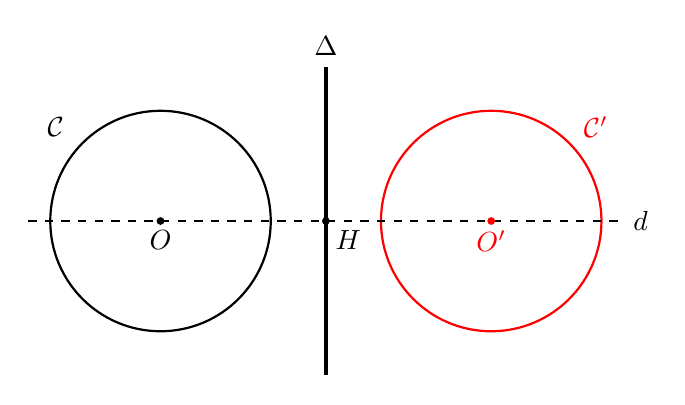
\begin{tikzpicture}[scale=0.7]
    \draw[very thick] (0,-2.8)--(0,2.8) node[above] {$\Delta$};
    \draw[thick] (-3,0) circle (2);
    \draw[thick,red] (3,0) circle (2);
    \draw[dashed] (-5.4,0)--(5.4,0) node[right] {$d$};
    \fill (-3,0) circle (2pt) node[below] {$O$};
    \fill[red] (3,0) circle (2pt) node[below] {$O'$};
    \fill (0,0) circle (2pt) node[below right] {$H$};
    \node at (-4.9,1.7) {$\mathcal{C}$};
    \node[red] at (4.9,1.7) {$\mathcal{C}'$};
  \end{tikzpicture}
  \end{center}
  \item الشعاع $2\cm$ أصغر من بعد $O$ عن $\Delta$ ($3\cm$) ، إذن الدائرة $\mathcal{C}$ لا تقطع $\Delta$ : هي كلها في جهة $O$.

  وبنفس الطريقة $\mathcal{C}'$ كلها في جهة $O'$ ، أي في الجهة الأخرى من $\Delta$.

  إذن \ib{لا توجد نقطة مشتركة} بين $\mathcal{C}$ و $\mathcal{C}'$.
  \item $d$ يمرّ من $O$ وهو عمودي على $\Delta$. والمستقيم $(OO')$ عمودي على $\Delta$ أيضا، ويمرّ من $O$ : إذن $d=(OO')$.

  $d$ يقطع $\Delta$ في $H$ ، ومناظرة $H$ هي $H$. ومناظرة $O$ هي $O'$ ، وهي على $d$.

  مناظر $d$ هو المستقيم المارّ من $H$ و $O'$ ، أي \ib{$d$ نفسه}.

  \textbf{انتبه :} كل مستقيم عمودي على المحور هو مناظر نفسه (لكن نقاطه تتبادل).
\end{enumerate}
\end{corr}

\end{document}
